\documentclass[../main]{subfiles}
\ifSubfilesClassLoaded{
    \dominitoc
    \tableofcontentsfile
    \pagenumbering{arabic}
    \setcounter{page}{1}
	\setcounter{chapter}{2}
}{}
\begin{document}
\chapter{Convergence de la relaxation}
\graphicspath{{./},{07-Relaxation/}}
\minitoc

\section{Introduction}

Le processus de relaxation que nous proposons dans l'algorithme CxSOM est une méthode originale pour construire des connexions bidirectionnelles entre cartes.
L'algorithme de relaxation proposé dans le modèle CxSOM s'appuie sur le modèle de relaxation que nous avions développé architectures de cartes auto-organisatrices cellulaires \cite{khouzam_neural_2014,menard05}.
Dans ces modèles d'architecture, le processus dynamique d'apprentissage s'appuie sur des champs neuronaux dynamiques couplés (DNF).
Ces champs dynamique approximent le comportement d'un champ de neurones impulsionnels
S'appuie sur des connexions excitatrices short range et inhibitrices à long terme -> winner take all style.
L'équivalent en SOM = BMU.
\cite{Kohonen1982} introduction des SOMs comme 
Ce processus cellulaire nécessite beaucoup de ressources de calcul~; l'algorithme de relaxation que nous proposons cherche à conserver un processus dynamique mais en le placant à l'échelle des cartes.

Deux cartes connectées de cette façon jouent alors un rôle symétrique.
La relaxation est en même temps une recherche d'un ensemble de Best Matching units par consensus.
Dans cette section, nous détaillons le formalisme de la méthode de relaxation que nous avons décrite de façon empirique et étudierons expérimentalement la relaxation sur un exemple d'apprentissage.


\section{Formalisme de l'algorithme de relaxation}

La recherche du BMU par consensus dans l'architecture CxSOM se traduit par une recherche du maximum des activations de toutes les cartes de l'architecture. La relaxation est une heuristique de recherche de ce maximum.

\subsection{Formalisation de l'algorithme de relaxation}

La relaxation définie dans le modèle est une recherche de maximum par déplacements dans l'espace des positions $(\bmu\m{1},\cdots, \bmu\m{n})$.
Nous notons $(\mathbf{\bmu})_\tau = (\bmu\m{0}_\tau,\cdots,\bmu\m{n}_\tau)$ la suite définie par l'évolution des BMUs des $n$ cartes d'une architecture lors de la relaxation.
Détaillons ici l'évolution de cette suite.

Pour clarifier les notations, nous définissons  pour chaque carte~$i$, une seconde suite $\hat{p}\m{i}_\tau$, correspondant à la position maximisant l'activité globale de la carte $i$ à l'instant $\tau$~:

\begin{equation}
\begin{gathered}
\hat{p}\m{i}_{\tau} = \argmax_p(a_g\m{i}(p,\bmu\m{i_0}_\tau, \cdots \bmu\m{i_K}_\tau))\\
 i_0, \cdots i_K \: \text{indices des cartes nourrissant la carte $i$}.
\end{gathered}
\label{eq:pstar}
\end{equation}

L'équation d'évolution de la suite $(\mathbf{\bmu})_\tau$ s'écrit à partir des valeurs $\hat{p}_\tau$: 
\begin{equation}
\bmu\m{i}_{\tau+1} = 
\begin{cases}
\bmu\m{i}_{\tau} + sgn(\hat{p}\m{i}_{\tau} - \bmu\m{i}_{\tau}) \times \delta \; & \text{si $\hat{p}\m{i}_{\tau} - \bmu\m{i}_{\tau} > \delta$ } \\
\hat{p}\m{i}_{\tau} \; \text{sinon}	
\end{cases}
\label{eq:evolution}
\end{equation}

$a_g\m{i}$ est une fonction des poids de la carte $\w\ext\m{i}, \w\cont\m{i}$ et de son entrée externe $\inpx\m{i}$. 
Lors du processus de relaxation, les poids et l'entrée $\inpx\m{i}$ restent fixes. 
Le calcul de $a_g$ à l'instant $\tau$ ne dépend donc pas de $\tau$. Pour toute carte $i$, $\hat{p}\m{i}_{\tau}$ dépend donc uniquement de $(\bmu\m{i_0}_\tau, \cdots \bmu\m{i_K}_\tau)$. 
% Notons que nous avions défini une première version de l'algorithme de relaxation dans laquelle les déplacements de $\bmu_\tau$ dépendent de leur distance à $\hat{p}_\tau$ : 

En posant $f\m{i}$ la partie droite de l'équation \ref{eq:evolution}, on peut donc écrire~: 
\begin{equation}
\forall i, \; \bmu\m{i}_{\tau +1} = f\m{i}(\bmu\m{0}_\tau,\cdots,\bmu\m{n}_\tau)
\label{eq:fonction}
\end{equation}

Soit, pour l'ensemble des composantes: 
\begin{equation}
\mathbf{\bmu}_{\tau+1} = \mathbf{f}(\mathbf{\bmu}_\tau)
\end{equation}

Si $(\bmu)_\tau$ converge, alors elle converge vers un point fixe de la fonction $f$, soit une position $\mathbf{\bmu}$ vérifiant~:

\begin{equation}
\mathbf{\bmu} = \mathbf{f}(\mathbf{\bmu})
\label{eq:suite}
\end{equation}

Les points fixes $\mathbf{\bmu}$ de la fonction $\mathbf{f}$ sont les valeurs maximisant le problème~\ref{eq:opti}.

Cependant, rien ne garantit que ces point fixes existent ni que la suite converge.
Pour des poids quelconques, ce n'est pas le cas. Il est donc pertinent d'observer le comportement de la relaxation dans le cas de cartes de Kohonen.

Notons enfin que l'évolution de la suite $(\mathbf{\bmu})_{\tau}$ dépend de son initialisation.
Lors de l'apprentissage du modèle, nous prenons comme état initial une position $(\bmu\m{0}_0, \cdots , \bmu\m{n}_0)$  telle que~: 
\begin{equation}
\begin{cases}
\bmu\m{0}_0 = \argmax_{p\m{0}} a_e(p\m{0},\inpx\m{0})\\
\cdots \\
\bmu\m{n}_0 = \argmax_{p\m{n}} a_e(p\m{n},\inpx\m{n})\\
\end{cases}
\label{eq:init}
\end{equation}

Nous étudierons dans ce chapitre la relaxation pour $(\bmu\m{0}_0, \cdots , \bmu\m{n}_0)$ quelconques.

\subsection{Formulation du problème d'optimisation}

La relaxation que nous venons de formaliser est la recherche d'un ensemble de valeurs que nous notons $\mathbf{\bmu} = (\bmu\m{1}, \cdots, \bmu\m{n})$.
Il s'agit d'une heuristique de recherche d'un maximum de l'activité totale de l'architecture, que nous détaillons ici.

Rappelons les équations de calcul d'activation~:
Dans chaque carte $i$, l'activité globale est définie par~:
\begin{equation}\label{eq:ag}
	a_g\m{i}(p, \inpx, \inpc_0, \cdots, \inpc_K) = \sqrt{a_e(p,\inpx)(\frac{1}{2}a_e(p,\inpx) + \frac{1}{2}a_c(p,\inpc_0, \cdots, \inpc_K)}
\end{equation}
Avec $\inpc_0, \cdots, \inpc_K$ les entrées contextuelles de la carte.

L'activité contextuelle $a_c$ est définie comme la moyenne des activités contextuelles sur chaque couche de poids contextuels~:
\begin{equation}
	a_c(p, \inpc_{i_0}, \cdots, \inpc_{i_K}) = \frac{1}{k+1}\sum_{k=0}^{K}{a_{ck}(p, \inpc_{i_k})}
\end{equation}

$a_g\m{i}$ étant à valeurs positives pour tout $i$, la recherche de BMU s'exprime comme une solution $(\bmu\m{0}, \cdots, \bmu\m{n})$ du problème d'optimisation suivant~:

\begin{equation}\label{eq:opti}
	\begin{cases}
	\text{Maximiser}\;& \sum_{i = 1}^n a_g\m{i}((\bmu\m{i},\inpx\m{i},\inpc_0\m{i}, \cdots, \inpc_n\m{i})) \\
	\text{Sous Contrainte }\; &\forall i,\:\forall k, \; \inpc_k\m{i} = \argmax_{p}a_g\m{k}(p,\inpc_0\m{k}, \cdots, \inpc_n\m{k})
	\end{cases}
\end{equation}

Les solutions du problème~\ref{eq:opti} sont les positions $(\bmu\m{1}, \cdots, \bmu\m{n})$ vérifiant~:
$$\bmu\m{i} = \argmax_p a_g(p, \bmu\m{0}, \cdots, \bmu\m{n})$$,c'est-à-dire les points fixes de la fonction $\mathbf{f}$ définie lors de la relaxation.

En fonction des poids des cartes, il n'est clairement pas assuré qu'une solution existe ni qu'elle soit unique. 
Dans un cas quelconque, ce problème n'a a priori pas de solution.
Nous observerons dans la suite que lorsque les poids des cartes présentent une continuité (au sens des cartes de Kohonen), le problème admet une solution.
Maintenant que nous avons posé un formalisme sur l'algorithme de relaxation, le but de ce chapitre est de visualiser la relaxation sur un exemple d'expérience.

\subsection{Relaxation et notion de \emph{Best Matching Unit}}

La notion de Best Matching Unit est définie au sein de l'algorithme d'apprentissage d'une carte de Kohonen, comme l'unité possédant l'activité maximale pour une entrée fixée. 
Cette activité dépend de l'entrée présentée et des poids de la carte, mais peut aussi dépendre d'autres variables pour d'autres modèles de carte, tels que l'état de la carte au temps précédent pour les cartes récurrentes, ou dans notre cas les positions des BMU des cartes adjacentes.

On attend d'un algorithme de recherche du BMU que la valeur trouvée en sortie soit uniquement relative aux poids de la carte et aux entrées~: elle ne doit pas dépendre de l'initialisation.
Dans le cas de la recherche de BMU par relaxation, nous voulons ainsi vérifier que~:

\begin{itemize}
	\item La recherche du BMU converge. S'il n'existe pas de point de convergence, nous ne pouvons pas définir un BMU pour la carte. Nous mesurerons pour cela la convergence de la relaxation sur un ensemble d'expériences.
	\item La valeur trouvée à l'issue de la relaxation, à savoir le point de convergence s'il existe, ne dépend pas des conditions initiales de la relaxation. 
	Le BMU est alors relatif à seulement l'état des poids de la carte et non des conditions initiales. Nous voulons donc vérifier que la fonction $\mathbf{f}$ générant la suite $\mathbf{\bmu}_\tau$ admet un unique point fixe.
\end{itemize}
L'évaluation de ces deux conditions sera réalisée sur des exemple d'apprentissage d'une architecture de deux et trois cartes. 
Notons que dans l'algorithme CxSOM, les BMUs sont initialisés à la position du maximum de l'activité externe dans chaque carte. 
Nous effectuerons l'analyse de la relaxation pour des conditions initiales quelconques, mais il est important de noter que ce choix d'initialisation permettra en fait d'éviter certains cas de non-convergence.

Nous montrerons expérimentalement qu'il n'existe pas toujours un unique point fixe, en particulier lorsque les poids sont répartis aléatoirement au début de l'apprentissage, ce qui entraîne alors une non-convergence de la relaxation. 
Cependant, nous observons que ces cas de non-convergence n'influencent pas le dépliement ultérieur des cartes, ce qui est permis par l'initialisation de la relaxation à la position maximisant l'activité externe.
Nous observerons expérimentalement qu'à la fin de l'apprentissage, la disposition des poids obtenue dans chaque carte permet l'existence d'un unique point fixe et que la relaxation converge vers ce point, indépendamment de l'initialisation des valeurs de $\bmu\m {i}_{\tau}$.

Ce chapitre présente des points d'analyse empirique de ce processus de relaxation, réalisée sur des cartes 1D et 2D prenant en entrée un jeu de données 1D.

La démarche expérimentale est la suivante:
Nous mesurerons d'abord la convergence de la relaxation dans les expériences citées ci-dessus.
Nous chercherons à observer à partir de deux visualisations l'unicité du point fixe et les trajectoires de la suite $\mathbf{\bmu}_\tau$ en fonction de l'initialisation de la relaxation.
Enfin, nous étudierons comment le choix du pas de relaxation $\Delta$ influence la convergence de la relaxation.

\section{Etude expérimentale de la convergence de la relaxation}

Nous nous intéressons ici  à un processus d'apprentissage complet d'une architectures de deux cartes. Les entrées $\inpx\m{1}$ et $\inpx\m{2}$ que nous présentons à chaque carte sont les coordonnées $x$ et $y$ de points situés sur un cercle de centre 0.5 et de rayon 0.5. 
Nous détaillerons le choix de disposition d'entrées dans les chapitres suivants~; notons simplement que ces entrées sont normalisées, chaque prenant toutes les valeurs entre 0 et 1. 

Pendant l'apprentissage, nous effectuons des phases de test régulières, à poids figés, sur 5000 points tirés selon les mêmes distributions d'entrées. 
Nous comptons ensuite, pour chaque entrée de test, le nombre de pas nécessaires avant la convergence de la relaxation. Lors des tests, nous initialisons la relaxation à la position maximisant l'activité externe.

En pratique, l'algorithme de relaxation s'arrête si la relaxation dépasse $\tau_{max}= 1000$ itérations~; nous considérerons donc que la relaxation n'a pas atteint un point de convergence si le nombre de pas de relaxation a atteint ces $\tau_{max}$ itérations lors de l'expérience. 
\'A partir de ces valeurs, nous pouvons traçer le nombre de pas moyen nécessaires à la convergence (en prenant en compte les cas dans lesquel la relaxation ne converge pas), ainsi que le taux de convergence~: la proportion d'entrées sur les 5000 entrées tests pour lesquelles la relaxation a convergé.
Nous répétons 10 fois l'apprentissage complet et les tests, sur les mêmes distributions d'entrée.
Nous réalisons ces expériences sur des cartes 1D et des cartes 2D.
Nous traçons en figure~\ref{fig:conv_evolution} la moyenne et l'écart type du nombre moyen de pas de relaxation et du taux de convergence obtenues sur ces 10 répétitions. La figure~\ref{fig:conv_evolution2D} présente ces valeurs obtenues avec des cartes 2D.

Plusieurs situations peuvent se traduire par une non-convergence de la relaxation:
\begin{itemize}
\item La relaxation évolue vers un point de convergence, mais trop lentement pour y arriver en moins de 1000 itérations
\item La relaxation évolue vers un cycle limite composé d'un nombre réduit d'unités se succédant alternativement
\item La relaxation évolue sans répétition d'un motif dans chaque carte~; il s'agit d'une évolution chaotique.
\end{itemize}

Le premier cas est évité car la limite de 1000 itérations est assez grande par rapport à la taille de la carte, les cartes sont de taille 500 et le pas d'évolution de la relaxation d'une dizaine d'unités. 
La convergence, si elle existe, est rapide. Les cas de non-convergence concernent alors la deuxième et la troisième situation. Nous observerons plus précisément les trajectoires dans la section suivante; on s'intéresse ici seulement à la question de la convergence.

Les figures~\ref{fig:conv_evolution} et \ref{fig:conv_evolution2D} montrent qu'au début de l'apprentissage, lorsque les poids sot initialisés aléatoirement, la relaxation atteint rarement un point de convergence. Lorsque les cartes sont dépliées, la relaxation évolue vers un point de convergence dans plus de $90 \%$ des cas. L'évolution est similaire pour des architectures de deux et trois cartes.

Nous en  concluons que la convergence de la relaxation dépend complètement de la disposition des poids. 
Elle converge dans plus de 90 \% des cas lorsque les poids sont bien dépliés, mais seulement dans 20\% des cas au début de l'apprentissage lorsque les poids ne présentent aucune forme de continuité et d'organisation.
Le fait que la relaxation ne converge pas en début d'apprentissage ne perturbe cependant pas l'organisation des poids.
Nous discuterons plus loin de cette observation.

\begin{figure}
\centering
\includegraphics[width=0.7\textwidth]{1D_conv_evolution_total.pdf}
\caption{En haut: évolution de la moyenne et l'écart-type du taux de convergence lors de la relaxation au cours de l'apprentissage sur deux et trois cartes 1D. En bas: évolution du nombre moyen de pas nécessaires à la convergence de la relaxation.
Chaque point est calculé sur un échantillon de 5000 relaxations au temps t, évaluées sur des entrées différentes prises aléatoirement sur le cercle. La moyenne et l'écart-type sont réalisés sur 10 apprentissages séparés.}
\label{fig:conv_evolution}
\end{figure}

\begin{figure}
	\centering
	\includegraphics[width=0.7\textwidth]{2D_conv_evolution_total.pdf}
	\caption{En haut: évolution de la moyenne et l'écart-type du taux de convergence lors de la relaxation au cours de l'apprentissage sur deux et trois cartes 2D. 
	En bas: évolution du nombre moyen de pas nécessaires à la convergence de la relaxation.
	Chaque point est calculé sur un échantillon de 1000 relaxations au temps t, évaluées sur des entrées différentes prises aléatoirement sur le cercle. La moyenne et l'écart-type sont réalisés sur 10 apprentissages séparés.}
	\label{fig:conv_evolution2D}
	\end{figure}

\section{\`Etude de l'évolution de la relaxation}

\subsection{Trajectoires de relaxation\label{sec:pf}}

Nous nous placons dans une architecture de deux cartes 1D.
Nous étudions dans cette partie l'évolution de plusieurs processus de relaxation lancés sur des poids de cartes dans une même disposition, à présent en fixant l'entrée externe et en prenant des valeurs d'initialisation de relaxation $\mathbf{\bmu}_0$ différentes.


Pour une architecture de deux cartes 1D, nous avons donc~:
\begin{equation*}
	\begin{cases}
	\hat{p}\m{1}_\tau = \argmax_p(a_g\m{1}(p, \bmu\m{2}_\tau))\\
	\hat{p}\m{2}_\tau = \argmax_p(a_g\m{1}(p, \bmu\m{1}_\tau)) \\
	\end{cases}
	\end{equation*}
et 

\begin{equation*}
	\begin{cases}
	\bmu\m{1}_{\tau+1} = \bmu\m{1}_\tau \pm sgn(\hat{p}\m{1}_\tau - \bmu\m{1}_\tau)  \\
	\bmu\m{2}_{\tau+1} = \bmu\m{2}_\tau \pm sgn(\hat{p}\m{2}_\tau - \bmu\m{2}_\tau) \\
	\end{cases}
	\end{equation*}

Avec $\hat{p}\m{1}$ dépendant seulement de $\bmu\m{2}$ et inversement. 
Dans cette situation, nous pourrons tracer la trajectoire de $\mathbf{\bmu}_\tau$ dans l'espace $(p\m{1}, p\m{2})$.

Dans cette expérience, nous comparons les trajectoires de $\mathbf{\bmu}_\tau$ obtenues dans deux configurations de poids des cartes~: une configuration dans laquelle tous les poids sont répartis aléatoirement dans $[0,1]$, ce qui est le cas au début d'un apprentissage, et une configuration obtenue après apprentissage de l'architecture, dans laquelle les poids présentent une continuité.
Nous nous intéressons dans chaque configuration aux trajectoires et aux points d'arrivées de 200 relaxations, obtenues pour une même entrée $\inpx$ mais des valeurs d'initialisation $\mathbf{\bmu_0}$ différentes choisies aléatoirement parmi toutes les positions des cartes.
Pour un problème à deux cartes, il est peu coûteux de trouver par une recherche exhaustive les points fixes de la fonction $\mathbf{f}$ générant la suite des BMUs.
Nous visualiserons ainsi les trajectoires de relaxation dans l'espace $(p\m{1},p\m{2})$ superposées à la valeur selon  $(p\m{1},p\m{2})$ de $\lvert \hat{p}\m{1} - p\m{1} \rvert$ et $\lvert \hat{p}\m{2} - p\m{2}\rvert$. 
Nous regarderons s'il existe un unique point où ces deux quantités s'annulent, c'est à dire le point fixe de $f$, et vérifierons si les trajectoires de relaxation convergent vers ce point.

En figure \ref{fig:diff_relax_t1_notraj}, nous traçons les deux quantités $\lvert \hat{p}\m{1} - p\m{1} \rvert$ et $\lvert \hat{p}\m{2} - p\m{2}\rvert$ au début de l'apprentissage. Les positions annulant chacune des quantités sont marquées par les zones en violet sur chaque graphique.
Nous y faisons figurer uniquement les positions de fin de relaxation de $(\bmu\m{1},\bmu\m{2})$ pour plus de lisibilité. Ces positions sont marquées par les points noirs.
Nous remarquons une position en $(0.1, 0.75)$, dans lequels les deux quantités sont nulles. Ce point fixe apparaît comme un hasard du choix des poids.
Nous observons que certaines trajectoires ont convergé vers cette position~: nous observons des points noirs a cet emplacement, mais que d'autres trajectoires ont amené la suite des BMUs vers d'autres positions.
Nous observons la présence de plusieurs cycles limites~: certaines trajectoires ne convergent pas et évoluent sur un cycle de positions.
Afin de mieux représenter les trajectoires, nous traçons également en \ref{fig:champ_0} le champ des déplacements de $(\bmu\m{1}_\tau,\bmu\m{2}_\tau)$ lors de la relaxation en fonction de la position courante. 
Nous y superposons les trajectoires aboutissants aux points présentés en figure \ref{fig:diff_relax_t1_notraj}.
Ces champs de déplacement permettent d'observer les comportements de point fixe et cycles limite des suites de BMUs.

La configuration en fin de l'apprentissage est présentée en figure~\ref{fig:diff_relax_notraj}. Nous y ajoutons cette fois 10 exemples de trajectoires de BMUs.
Une structure apparaît dans les valeurs des différences, et un point où les deux différences sont nulles existe à l'intersection des deux zones violettes.
Sur ces tracés, nous observons un seul point d'attraction pour les 200 trajectoires. La relaxation ne dépend donc plus des conditions initiales.
Ce point correspond à la position où les deux différences $\lvert \hat{p}\m{1} - p\m{1} \rvert$ et $\lvert \hat{p}\m{2} - p\m{2}\rvert$ sont nulles.
La figure \ref{fig:champ_9999} présente le champ de déplacement des BMUs en fonction de la position courante. Les trajectoires suivent les zones où l'une ou l'autre des différences est nulle, pour mener à la position stable. 


Cette propriété vient de la disposition ordonnée des poids externes à la fin de l'apprentissage et de la formule du calcul d'activité.
\'A la fin de l'apprentissage, $a_e(\inpx,p)$ présente un seul maximum. 
De plus, l'activité globale correspond à la modulation de l'activité contextuelle par les valeurs de l'activité externe. Donc, à $\inpx\m{1}$ fixé ,$\hat{p}\m{1} = \argmax_p\m{1} a_g(p\m{1}, p\m{2})$ reste dans une zone restreinte lorsque $p\m{2}$ varie (de même pour $a_g\m{2}$). 
La relaxation évoluera donc vers cette zone réduite.
Cette propriété est illustrée en figure\ref{fig:w006}.
Nous y faisons figurer les poids des deux cartes et les valeurs de $\hat{p}\m{1}$ et $\hat{p}\m{2}$ obtenues en faisant varier $p\m{1}, p\m{2}$ dans tout l'espace des positions possibles.

D'après cet exemple, nous formulons l'hypothèse que le dépliement ordonné des poids externes dans une carte en 1D est une condition suffisante à l'existence d'un unique point fixe. 
Dans ce cas, la relaxation permet de trouver ce point fixe.


\begin{figure}
\begin{minipage}{0.5\textwidth}
\centering
\includegraphics[width=\textwidth]{champ_X_006_t1_notraj.pdf}
\end{minipage}
\begin{minipage}{0.5\textwidth}
\centering
\includegraphics[width=\textwidth]{champ_Y_006_t1_notraj.pdf}
\end{minipage}
\caption{Valeur de ${\hat{p}}\m{1} - p\m{1}$, resp. ${\hat{p}}\m{2} - p\m{2}$ à $t=0$ ,lorsque les poids sont encore aléatoiremement disposés dans chaque carte.
 ${\hat{p}}\m{1}$ ne dépend que de $p\m{2}$ : on peut donc tracer cette valeur selon deux dimensions pour chaque carte. Les zones où cette valeur est nulle sont en violet sur le graphique. Les points fixes, s'il existent, sont aux positions de différence nulle pour $M\m{1}$ et $M\m{2}$. Les points noirs représentent les points de convergence pour 200 trajectoires de relaxation, lancées pour différents $\bmu_0\m{1}, \bmu_0\m{2}$.}
 
\label{fig:diff_relax_t1_notraj}
\end{figure}

\begin{figure}
\begin{minipage}{0.5\textwidth}
\centering
\includegraphics[width=\textwidth]{champ_X_006.pdf}
\end{minipage}
\begin{minipage}{0.5\textwidth}
\centering
\includegraphics[width=\textwidth]{champ_Y_006.pdf}
\end{minipage}
\caption{Valeur de ${\hat{p}}\m{1} - p\m{1}$, resp. ${\hat{p}}\m{2} - p\m{2}$, lorsque les cartes sont organisées telles qu'en figure \ref{fig:w006}. ${\hat{p}}\m{1}$ ne dépend que de $p\m{2}$ : on peut donc tracer cette valeur selon deux dimensions pour chaque carte. Les zones où cette valeur est nulle sont en violet sur le graphique. Les points fixes, s'il existent, sont aux positions de différence nulle pour $M\m{1}$ et $M\m{2}$. Les points noirs représentent les points d'arrivée de la relaxation pour 50 trajectoires de relaxation, lancées pour différents $\bmu_0\m{1}, \bmu_0\m{2}$. La relaxation semble présenter un point de convergence, qui se situe sur un point fixe de la fonction de relaxation.}
\label{fig:diff_relax_notraj}
\end{figure}

\begin{figure}
\centering
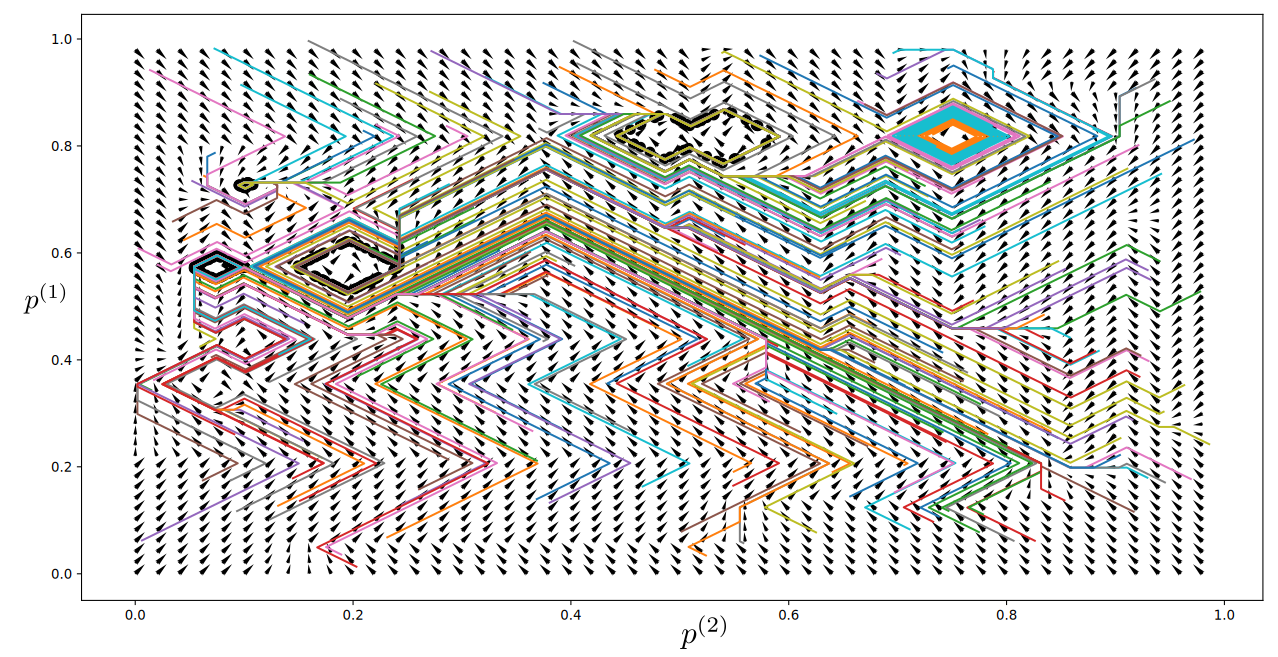
\includegraphics[width=\textwidth]{champ_006_t1.pdf}
\caption{Champ de déplacements de $\bmu\m{1},\bmu\m{2}$ lorsque les poids sont encore aléatoires, à $t=0$. Les trajectoires de 200 relaxations, initialisées différemment, sont représentées. En fonction de la position initiale des BMUs, la relaxation évolue vers un point fixe ou un cycle limite. }
\label{fig:champ_0}
\end{figure}


\begin{figure}
\centering
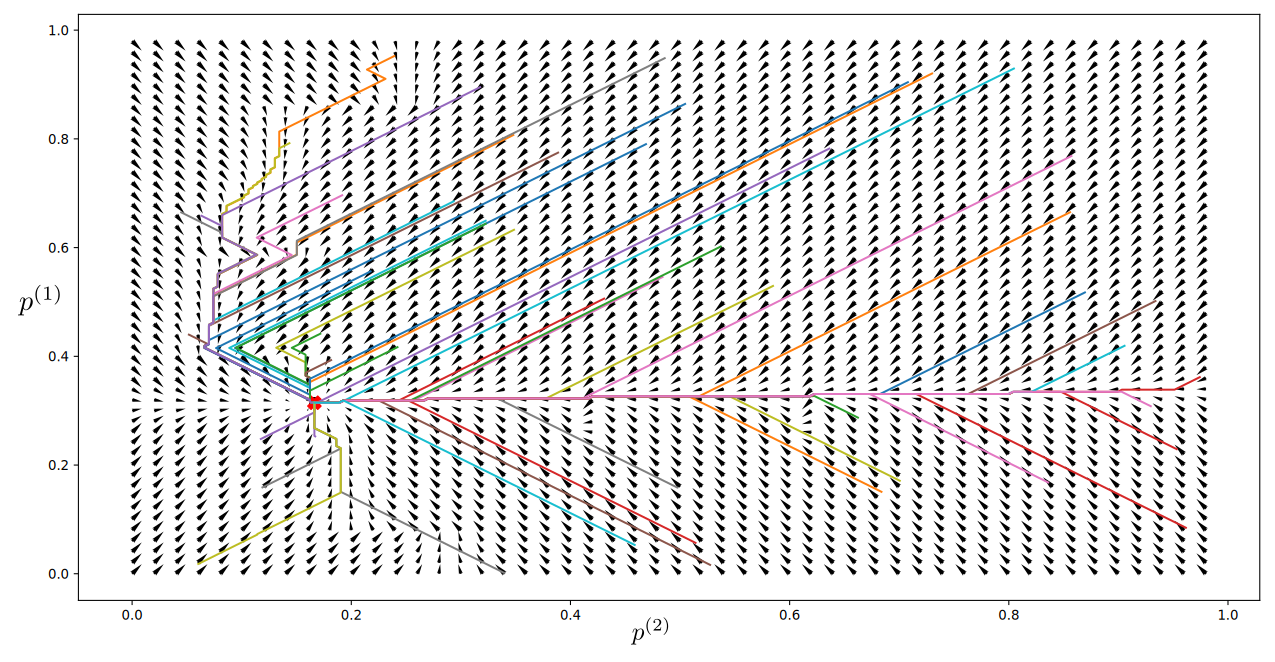
\includegraphics[width=\textwidth]{champ_006.pdf}
\caption{Champ de déplacements de $\bmu\m{1},\bmu\m{2}$ lorsque les poids sont organisés tels que représentés en figure \ref{fig:w006}, à $t=9999$.es trajectoires de 50  relaxations, initialisées différemment, sont représentées. Les relaxations évoluent vers un point fixe commun.}
\label{fig:champ_9999}
\end{figure}

\begin{figure}
	\includegraphics[width=\textwidth]{am_w_006}
	\caption{(a): $\hat{p}\m{1}$ et $\hat{p}\m{2}$ en fonction de l'entrée contextuelle de leur carte $\bmu\m{2}$ et $\bmu\m{1}$.(b): les poids externes et contextuels des cartes $1$ et $2$ sont représentés selon leur position dans la carte. On représente également les entrées test $\inpx\m{1}$ et $\inpx\m{2}$ en fonction de leur BMU. Les entrées utilisées pour tracer les figures de gauche sont colorées en rouge sur les figure de droite: $\inpx\m{1}=0.26,\inpx\m{2}=0.06$. Les intervalles dans lequel les valeurs de $\hat{p}$ varient sont reportés sur la figure (b).}
	\label{fig:w006}
	\end{figure}

\subsection{Influence du pas de relaxation}

Dans les expériences précédentes, nous avons utilisé un pas de convergence $\delta=0.05$.
Une autre solution est de ne pas utiliser de pas de relaxation, c'est à dire, à chaque itération, déplacer le BMU $\bmu\m{i}_\tau$ directement en $\hat{p}\m{i}$, où l'activité globale est maximale, au lieu de le déplacer de $\delta$.
L'évolution de la relaxation devient alors:
\begin{equation}
\forall i, \bmu\m{i}_{\tau+1} = \hat{p}\m{i}_{\tau}
\end{equation}

En figure \ref{fig:diff_nopas}, Nous avons tracé différentes trajectoires de relaxation, pour une même entrée. 
On représente sur cette même figure les différences ${\hat{p}}\m{1} - p\m{1}$ et ${\hat{p}}\m{2} - p\m{2}$. Le point fixé de la fonction génératrice de la suite $(\bmu)_\tau$ est un point pour lequel les deux valeurs sont nulles.
Ces relaxation sont effectués après l'apprentissage des données par l'architecture. La méthode de relaxation utilisée lors de l'apprentissage n'utilise pas non plus de pas de relaxation $\delta$.
A l'issue de l'apprentissage, le comportement de la relaxation ne change pas. 
Cela se comprend au vu des résultats précédents. $\hat{p}\m{1}$ et $\hat{p}\m{2}$ sont dans un intervalle réduit de valeurs de la carte, quelles que soient les positions $p\m{1}$ et $p\m{2}$. Amener directement le BMU dans cet intervalle ou l'y amener pas à pas ne change rien en terme de comportement. 

\begin{figure}
\begin{minipage}{0.5\textwidth}
\includegraphics[width=\textwidth]{champ_X_009}
\end{minipage}
\begin{minipage}{0.5\textwidth}
\includegraphics[width=\textwidth]{champ_Y_009}
\end{minipage}
\caption{Trajectoires des relaxations $(\bmu\m{1}_{\tau},\bmu\m{2}_\tau)$ dans le champ des différences ${\hat{p}}\m{1} - p\m{1}$ et ${\hat{p}}\m{2} - p\m{2}$, lorsque la relaxation est effectuée sans utiliser de petits déplacements. Les tracés sont effectués après apprentissage. La relaxation semble encore converger vers un point fixe.}
\label{fig:diff_nopas}
\end{figure}

\section{Conclusion}

Les parties \ref{sec:conv} et \ref{sec:cont} montrent donc que, lorsque les poids sont quelconques, la convergence de l'algorithme de relaxation n'est pas assurée; au contraire, la relaxation évolue dans la plupart des cas vers une situation non convergente. Dans le cas particulier étudié dans la section, il semble exister des point fixes, mais dus au caractère aléatoire des poids. La relaxation ne permet pas de trouver ces points. Pourtant, l'apprentissage des cartes utilisant la relaxation comme recherche de BMU mène une organisation des poids, même sans que la relaxation ne converge au début. Cette organisation permet de plus une meilleure convergence de la relaxation (convergence dans plus de $90 \%$ des cas).

Ce comportement peut être expliqué. On observe que la relaxation converge bien à partir du moment où les poids externes sont organisés et présentent une continuité. 
Au début de l'apprentissage, même si la relaxation mène à des positions quelconques de BMUs, ces BMUs auront quand même des poids externes restant proches de la valeur de l'entrée externe. 
Le calcul de l'activité dépend en effet d'abord de l'activité externe de la carte:
$$ a_g = \sqrt{a_e ( \beta a_e + (1-\beta a_c))}, \;\; \beta=0.5$$ 
De plus, la relaxation est initialisée à une position correspondant au maximum de l'activité externe.

L'organisation de la carte s'effectuera donc de façon similaire à une carte classique. Dans une carte de Kohonen, pour des poids aléatoires, de multiples positions de BMU sont possibles lors du calcul de la distance des poids à l'entrée. La disposition des poids et le choix du BMU n'influencent pas la propriété globale d'organisation d'une carte. Cette même observation peut s'effectuer ici. 
Le rayon de voisinage externe étant bien plus grand que le rayon de voisinage contextuel, l'organisation des poids externes de la carte influence peu l'organisation des poids contextuels.
Lorsque les poids externes présentent une continuité, la relaxation converge. Les poids contextuels peuvent alors s'organiser selon le BMU, qui a maintenant un sens: il s'agit d'un point fixe de la fonction de relaxation. Le BMU correspond alors au point qui maximise en même temps les activités globale de chaque carte.

Expérimentalement, on observe que, lorsque les cartes sont organisés, le point fixe  existe, est unique est est atteint par n'importe quelle trajectoire de relaxation. Le BMU a donc un sens au niveau de la carte. 

Enfin, la relaxation utilise un pas de déplacement utilisé $\delta$. 
On pourrait supposer que prendre un petit $\delta$ permet une meilleure convergence; en fait, la valeur de $\delta$ influence peu la capacité de convergence et l'organisation des cartes. La relaxation pourrait être effectuée sans utiliser de pas de relaxation. Par ailleurs, la relaxation est initialisée proche de la position théorique du BMU, quand elle existe. La relaxation est donc finalement assez courte.

La relaxation est donc une recherche d'un maximum global à l'architecture, ce maximum étant un point fixe de la fonction de mise à jour des positions.
Une fois que les poids externes d'une carte présentent une continuité, la relaxation et le BMU issu de ce processus ont un sens topologique: on observe expérimentalement que la fonction de mise à jour présente un point fixe $\mathbf{\bmu} = \mathbf{f}(\mathbf{\bmu})$, et que la relaxation converge vers ce point fixe. Ce point fixe est alors le point qui maximise \emph{collectivement} les activités globales de chaque carte de l'architecture.
Bien que la relaxation ne converge pas au début de l'apprentissage, la convergence est observée dès que les poids externes présentent une certaine continuité. Cette continuité étant assurée après quelques itérations d'apprentissage par l'algorithme de mise à jours des poids de Kohonen, on peut donc dire que la relaxation converge au sein de CxSOM.
La relaxation est alors un moyen de trouver un ensemble de BMU au sein d'une architecture maximisant une propriété \emph{globale} à cette architecture: toutes les cartes voient leur activité globale maximisée. 
Cette recherche de maximum est réalisée localement, au niveau de chaque carte, et non de façon globale. La relaxation agit alors comme une manière de connecter des cartes de façon non-hiérarchique et les BMUs sont l'interface entre modules de la carte.

\ifSubfilesClassLoaded{
    \printbibliography
    %\externaldocument{../main.tex}   
}{}
\end{document}
